\documentclass[a4paper]{article}
\usepackage[a4paper,hmargin={3cm,2.5cm},vmargin={2.5cm,2.5cm}]{geometry}

\usepackage{tikz}
\usetikzlibrary{calc}

\usepackage{fancyhdr}
\pagestyle{fancy}
\lhead{}
\rhead{Detection of Cipher Types using Artificial Neural Networks}
\lfoot{Department of Computer Science an Technology}

\usepackage{lipsum}

\usepackage{multicol}

\usepackage{ragged2e}

\usepackage{xcolor}

\usepackage{enumitem}

\usepackage{caption}
\usepackage{subcaption}

\usepackage{listings}
\definecolor{mygreen}{rgb}{0,0.6,0}
\definecolor{mygray}{rgb}{0.5,0.5,0.5}
\definecolor{mymauve}{rgb}{0.58,0,0.82}

\lstset{
    backgroundcolor=\color{white},      % choose the background color; you must add \usepackage{color} or \usepackage{xcolor}; should come as last argument
    language=Python,                    % the language of the code
    basicstyle=\footnotesize\ttfamily,  % the size of the fonts that are used for the code
    breakatwhitespace=false,            % sets if automatic breaks should only happen at whitespace
    breaklines=true,                    % sets automatic line breaking
    captionpos=b,                       % sets the caption-position to bottom
    commentstyle=\color{mygreen},       % comment style
    deletekeywords={\ldots},            % if you want to delete keywords from the given language
    escapeinside={\%*}{*},              % if you want to add LaTeX within your code
    extendedchars=true,                 % lets you use non-ASCII characters; for 8-bits encodings only, does not work with UTF-8
    firstnumber=1,                      % start line enumeration with line 1
    numbers=left,                       % where to put the line-numbers; possible values are (none, left, right)
    numberstyle=\tiny\color{mygray},    % the style that is used for the line-numbers
    numbersep=7pt,                      % how far the line-numbers are from the code
	frame=single,                       % code snippet frame, t-> top, b->bottom, l->left, r->right, single-> all around
	tabsize=4,                          % tab = (tabsize) * space
    columns=flexible,                   % two options, fixed or flexible
    keepspaces=true,                    % keeps spaces in text, useful for keeping indentation of code (possibly needs columns=flexible)
    morekeywords={*,\ldots},               % if you want to add more keywords to the set
    rulecolor=\color{black},            % if not set, the frame-color may be changed on line-breaks within not-black text (e.g. comments (green here))
	showspaces=false,                   % show spaces everywhere adding particular underscores; it overrides 'showstringspaces'
    showstringspaces=false,             % underline spaces within strings only
    showtabs=false,                     % show tabs within strings adding particular underscores
    stepnumber=1,                       % the step between two line-numbers. If it's 1, each line will be numbered
    stringstyle=\color{mymauve},        % string literal style
    title=\small\lstname,                     % show the filename of files included with \lstinputlisting; also try caption instead of title
	% keepspaces,
	keywordstyle=\color{blue}           % keyword style    
}

\usepackage{hyperref}

\begin{document}
\begin{titlepage}
    \begin{tikzpicture}[overlay,remember picture]
        \draw[line width=4pt]
        ($ (current page.north west) + (1cm,-1cm) $)
        rectangle
        ($ (current page.south east) + (-1cm,1cm) $);
        \draw[line width=1.5pt]
        ($ (current page.north west) + (1.2cm,-1.2cm) $)
        rectangle
        ($ (current page.south east) + (-1.2cm,1.2cm) $);
    \end{tikzpicture}

    \begin{center}

        \textup{\large  \textbf{INDIAN INSTITUTE OF ENGINEERING}\\\textbf{SCIENCE AND TECHNOLOGY, SHIBPUR}}\\ Howrah, West Bengal, India – 711103\\[0.5cm]\textbf{\large DEPARTMENT OF COMPUTER SCIENCE}\\\textbf{\large AND TECHNOLOGY}

        %---------------------------------Figure------------------------------
        \begin{center}
            \begin{figure}[h]   %h means here other options t , b, p, etc.
                \centering
                
\includegraphics[width=0.3\linewidth]{Pictures/IIESTS_Logo.png}
            \end{figure}
        \end{center}

        %----------------------------

        \textup{\large A PROJECT REPORT SUBMITTED IN PARTIAL FULFILLMENT OF THE REQUIREMENTS\\[0.4cm]ON}\\[0.4cm]

        \begin{LARGE}
            \textbf {“DETECTION OF CIPHER TYPES USING}\\
            [0.2cm]
            \textbf {ARTIFICIAL NEURAL NETWORKS”}
        \end{LARGE}\\[1cm]

        \textit{SUBMITTED BY}\\[0.3cm]
        \begin{large}
            \textbf{Rajdeep Ghosh (510519002)}\\[0.1cm]
            \textbf{Swarnali Mondal (510510103)}\\[0.1cm]
            \textbf{Krishnendu Bera (510519004)}\\[0.1cm]
            \textbf{Arnab Sen (510519006)}\\[0.1cm]
            \textbf{Sanjana Chakravarty (510519038)}\\[0.1cm]
            \textbf{Abhiroop Mukherjee (510519109)}\\[1cm]
        \end{large}

        \textit{UNDER THE GUIDANCE OF}\\[0.5cm]
        \begin{large}
            \textbf{DR.\@ MALAY KULE}\\[0.3cm]
        \end{large}

        \textbf{(Academic Year: 2022–2023)}
    \end{center}
\end{titlepage}
%================begin of certificate page======================

\begin{titlepage}
    \begin{tikzpicture}[overlay,remember picture]
        \draw[line width=4pt]
        ($ (current page.north west) + (1cm,-1cm) $)
        rectangle
        ($ (current page.south east) + (-1cm,1cm) $);
        \draw[line width=1.5pt]
        ($ (current page.north west) + (1.2cm,-1.2cm) $)
        rectangle
        ($ (current page.south east) + (-1.2cm,1.2cm) $);
    \end{tikzpicture}

    \begin{center}
        \textup{\large  \textbf{INDIAN INSTITUTE OF ENGINEERING}\\\textbf{SCIENCE AND TECHNOLOGY, SHIBPUR}}\\ Howrah, West Bengal, India – 711103\\[0.5cm]\textbf{\large DEPARTMENT OF COMPUTER SCIENCE}\\\textbf{\large AND TECHNOLOGY}

        %---------------------------------Figure------------------------------
        \begin{center}
            \begin{figure}[h]   %h means here other options t , b, p, etc.
                \centering
                
\includegraphics[width=0.3\linewidth]{Pictures/IIESTS_Logo.png}
            \end{figure}
        \end{center}

        %----------------------------


        \begin{LARGE}
            \textbf{\textit {Certificate}}
        \end{LARGE}\\[1.2cm]
    \end{center}

    It is certified hereby that this report, titled “Detection of Cipher Types using Artificial Neural Networks”, and all the attached
    documents herewith are authentic records of Rajdeep Ghosh (510519002), Swarnali Mondal (510510103), Krishnendu Bera (510519004),
    Arnab Sen (510519006), Sanjana Chakravarty (510519038), and Abhiroop Mukherjee (510519109) from the Prestigious Department of Computer Science And Technology
    of the Distinguished and Respected IIEST Shibpur under my guidance.

    The works of these students satisfy all the requirements for which it is submitted.
    To the extent of my knowledge, it has not been submitted to any different institutions for
    the award of a degree.

    \vspace{5cm}
    \begin{multicols}{2}
        \begin{center}
            \textbf{Dr.\ Malay Kule\\Asst. Professor}\hspace{5cm}
        \end{center}
        \begin{center}
            \textbf{Dr.\ Asit Kumar Das\\Head Of Department}
        \end{center}
        \vspace{0.5cm}
    \end{multicols}
    \vfill
\end{titlepage}
%================end of title page======================

%----------------------ACKNOWLEDGEMENT---------------------------
\pagebreak
\newpage

\begin{titlepage}
    \begin{center}
        {\Large{\bf{\textit{ACKNOWLEDGEMENT}}\\[2cm]}}
    \end{center}


    \paragraph{\normalfont\textit{\indent We, as the students of IIEST, consider ourselves honored to be working with Dr.\ Malay Kule and Mr.\ Subinoy Sikdar.
            The success of this project would not have been possible without his useful insights,
            appropriate guidance, and necessary criticism.}}
    \paragraph{\normalfont\textit{\indent We would pass our token of gratitude to the Department of Computer Science And Technology as well for providing
            us with the opportunity to be able to tackle real-world problems while improving
            our problem-solving ability and thinking capacity by organizing this project. We all have
            learned quite a handful of new skills and are eager to use them henceforth as well.}}

    \begin{flushleft}
        \textit{Rajdeep Ghosh (510519002)\\
            Swarnali Mondal (510510103)\\
            Krishnendu Bera (510519004)\\
            Arnab Sen (510519006)\\
            Sanjana Chakravarty (510519038)\\
            Abhiroop Mukherjee (510519109)
        }
    \end{flushleft}
\end{titlepage}

\pagenumbering{roman}
\setcounter{page}{1}
\newpage
\setcounter{tocdepth}{2} % + subsections
\tableofcontents
\lfoot{Dept.\ of Computer Science \& Technology}
\newpage

\pagenumbering{arabic}
\setcounter{page}{1}

%%%%%%%%% MAIN TEXT STARTS HERE %%%%%%%%%%
\section{INTRODUCTION}
Information is the power in the present day. 
Information and data should be protected from 
unauthorized access, distortion, or any 
unauthorized activity. 

Cryptography is the study of secret writing. Information is 
no longer hidden due to the existence of network adversaries. 
Our communication channel is completely unstable; a third 
party might covertly eavesdrop and obtain information from 
the network or from the channel. Here, cryptography is crucial 
in preventing unauthorized access to our data. Using key(s), 
cryptography converts plaintext messages into unreadable ciphertext 
and vice versa. Encryption is the process of employing a key(s) 
to transform the original message into an unintelligible format, 
while decryption is the act of using a key(s) to convert the 
cipher text back to plaintext. The messages can only be encrypted 
or decrypted by the authorized user.

The project's objective is to examine encrypted text files to 
find and categorize their cipher types using artificial neural 
networks. The cipher algorithm classification model is based 
on the steps: 
\begin{enumerate}
    \item   Creation of a collection of cipher texts with various cipher texts.
    \item   Building a Deep Neural Network (DNN) and training it with a variety of cipher texts and training parameters to enable accurate learning and cipher text classification. 
    \item   Using the trained model to determine the algorithm that might have been used to generate the cipher text. 
\end{enumerate}

\section{PRELIMINARIES}

To ramp up for this project, we needed a basic knowledge of neural networks and deep learning and an overview of the classical encryption algorithms that we would be targeting in this project. Having specific knowledge of the encryption algorithms will be useful to particularly train the model.

The ML topics that are covered in this project are:
\begin{itemize}
    \item Perceptron
    \item Artificial Neural Network (ANN)
    \item Recurrent Neural Network (RNN)
    \item Convolutional Neural Network (CNN)
    \item Transformers
    \item Attention Mechanism in Deep Learning
\end{itemize}

\newpage

\section{LITERATURE SURVEY}

Over recent years, artificial neural networks (ANNs) have 
come to prominence. Applications and research areas for ANNs are numerous and diverse. Their primary objective is the quick filtering, classification, and processing of (mainly) non-linear data, such as speech recognition, picture processing, and language translation. In addition, researchers were able to “train” ANNs to play games (e.g. AlphaStar \cite{AlphaStar:online}) or produce artwork in the manner of well-known artists.

On the MysteryTwister C3\cite{Welcomet7:online} (MTC3) website 
in late 2019, Stamp posted a challenge titled “Cipher ID”. The 
task is to identify the type of cipher used to encrypt each 
of the 500 ciphertexts in the collection, which were encrypted 
using 5 distinct ciphers and random keys. The individual ciphertexts 
were then mixed up after each cipher type had been employed 
exactly 100 times. All prior solvers completed the task by deciphering 
the ciphertexts using solvers for the 5 various cipher types, 
despite the author's goal of encouraging others to begin research 
in the fields of machine learning and cipher type detection. 
The participants were able to determine the type of encryption 
the algorithm that was employed after learning the plaintext of each cipher.

We worked on the cipher text detection problem with the help of ANN 
and in this process, TensorFlow and Pytorch were used. TensorFlow 
is a free and open-source data flow and math library developed 
by Google written in Python, C++, and CUDA, and was publicly
released in 2015. PyTorch is an open-source machine learning (ML) 
framework based on the Python programming language and the Torch 
library which was initially released in the year 2016.

In this section, we present different papers and articles, which 
we studied before starting with our work. The usage of ANNs 
in the paper ranges between the emulation of ciphers, the detection 
of the cipher type, and the recovery of cryptographic keys.

\begin{enumerate}
    \item Attention Is All You Need\cite{https://doi.org/10.48550/arxiv.1706.03762} 
    (NIPS 2017), here a new simple network architecture, the 
    Transformer, based solely on attention mechanisms, dispensing 
    with recurrence and convolutions entirely. Experiments on 
    two machine translation tasks show these models to be superior 
    in quality while being more parallelizable and requiring 
    significantly less time to train.
    \item Detecting the Type of Ciphers Using Artificial Neural 
    Networks\cite{inproceedings} (ICHC, 2020), where a first 
    version of an artificial neural network was developed to 
    differentiate between five classical ciphers: simple 
    monoalphabetic substitution, Vigenere, Playfair, Hill, and
    transposition.
    \item In the Language Models are Unsupervised Multitask 
    Learners\cite{radford2019language} paper, demonstration 
    of language models that can perform down-stream tasks in 
    a zero-shot setting – without any parameter or architecture 
    modification was done.
    \item Language Models are Few-Shot Learners\cite{brown2020language}, 
    broader societal impacts of this finding and of GPT-3 in 
    general are discussed in this paper
    \item Detection of Classical Cipher Types with Feature-Learning 
    Approaches\cite{leierzopf2021detection}, where the applicability 
    of the two feature-learning algorithms, long short-term 
    memory (LSTM) and Transformer, have been explored to overcome 
    the dependency on domain knowledge
    \item A systematic evaluation of large language models of 
    code\cite{xu2022systematic} (ICLR 2022), where a new model 
    PolyCoder was released, with 2.7B parameters based on the GPT-2
    architecture, that was trained on 249GB of code across 12 
    programming languages on a single machine.
    \item GPT-NeoX-20B:\@ An Open-Source Autoregressive Language 
    Model\cite{black2022gpt}, where GPT-NeoX-20B was introduced 
    which was a 20-billion-parameter autoregressive language model 
    trained on the Pile.
    \item Fine-tune a pretrained model\cite{Finetune56:online}, 
    a tutorial where a step-by-step process to fine-tune a
    pretrained model with a deep learning framework is discussed.
    \item Fine-Tuning Transformers for NLP\cite{FineTuni38:online}, 
    another tutorial on how to fine-tune two different transformer 
    models, BERT and DistilBERT:\@ Sentiment Analysis, and Duplicate
    Question Detection is covered.
    \item How to generate text: using different decoding methods 
    for language generation with
    Transformers~\cite{Howtogen29:online}, a blog post which 
    gives a brief overview of different decoding
    strategies and shows how can they be implemented with very 
    little effort using the popular transformers library
\end{enumerate}


\newpage

\section{PROPOSED WORK}
\subsection{Dataset Generation}
The dataset has been generated for five types of ciphers:
\begin{itemize}
    \item Caesar
    \item Affine
    \item Vigenère
    \item Substitution
    \item Rail Fence
\end{itemize}

The plaintext used for encryption was a text from Shakespeare’s Hamlet and Macbeth.

For Data Preprocessing, we converted text to lowercase and removed all whitespaces and punctuation.

Each of the classes has 6815 data points, resulting in a total 
of 34075 data points and each data point consists of the ciphertext 
(input) and the encryption algorithm (output).

We wrote a Python script for each of the ciphers to encrypt 
the data into a Pandas DataFrame. The combined DataFrame is shuffled and 
exported as a CSV file for the resulting dataset.

\subsection{Model using CNN}

The main intuition behind this method is that CNN uses its kernel as a “local receptive field”, which means that a CNN kernel (small in size as we are dealing with stream cipher and not block cipher) can look at its nearby characters and will find some pattern in the ciphertext

So, we first converted every ciphertext into their respective list of tokens using a  TextVectorizer, then we converted that list into a 2D text matrix as follows:

\begin{figure}[h!]
    \centering
    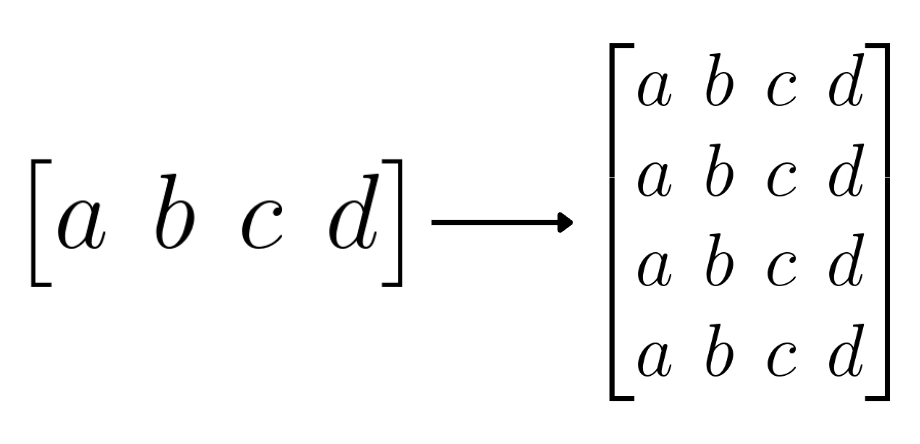
\includegraphics[width=0.4\linewidth]{Pictures/CNN_Model/string_conversion.png}
    \caption{Converting text to “image”}\label{fig1:convert_text_img}
\end{figure}

Note that this conversion depends on the length of the string used, i.e.\ for a string for length $n$, we will generate a $n \times n$ “image”. After we generate all variable-sized images, we resize them to $60 \times 60$ using Bilinear Interpolation.

Now we can see that a kernel (say $3 \times 3$ with stride one) 
can observe its previous as well as its next character and 
can use that information to find patterns in the ciphertext.

We use a CNN to extract features from the “image” and then we feed those features to a Dense Network to classify between the ciphertext types.

\newpage

\subsection{Model using Transformer}

The main intuition behind this method is to compute the relative 
importance of a ciphertext character with respect to the other 
ciphertext characters. A transformer model works on the encoder 
decoder architecture converting ciphertext characters to tokens 
and then computing the relative importance of a token to other tokens.

\begin{figure}[h!]
    \centering
    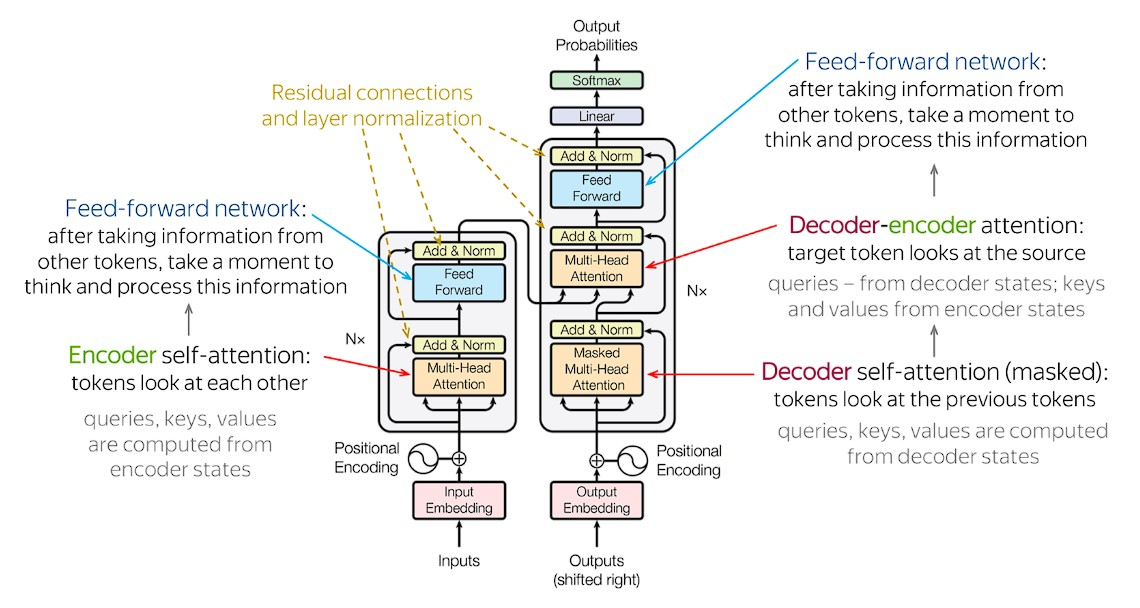
\includegraphics[width=\linewidth]{Pictures/Transformer_Model/transformer_arch.jpg}
    \caption{Transformer architecture}\label{fig2:transformer_arch}
\end{figure}

A transformer is an advanced sequence-to-sequence model that 
is used to predict the next token depending on all the previous 
tokens. From our dataset containing encrypted text and the algorithm 
used for encryption, we create a text prompt from each row for 
example: 
\begin{flushleft}
    Cipher text: \texttt{ymccaygimgamkyyiycuycqocyeagmigkycmyyoyy}\\
    Algorithm: \texttt{affine}
\end{flushleft}

The model learns the relative importance of each token and uses 
it to predict the next. For example, if the model is trained 
with the above prompt and then we supply the following prompt: 

\begin{flushleft}
    Cipher text: \texttt{ymccaygimgamkyyiycuycqocyeagmigkycmyyoyy}\\
    Algorithm: 
\end{flushleft}

The model shall generate the output as “affine” which it learned 
from training. 

In our use case, we have used the GPT-Neo (Generative Pre-Trained) model with 125 million parameters to achieve our objective.  It consists of stacks of encoders and decoders put one after the other, of which has been pre-trained on Wikipedia Corpus as well as Common Crawl (This has over 12 Petabytes of data which is 12 years of data uploaded on the internet) datasets for performing extremely well on language-based use cases. Generative, as the word suggests, is for making our code generate text. The architecture is similar to GPT2 except that GPT Neo uses local attention in every other layer with a window size of 256 tokens. All these models are available for free in the Hugging Face transformers library which can be used for a variety of NLP tasks.

\newpage

The following steps were taken for this model:
\begin{enumerate}
    \item   Each data of the dataset is converted into text prompts 
            that is passed through a tokenizer that creates embeddings 
            for each token in our input string. 
    \item   The input dataset has been split into the ratio 
            80:10:10 for training, testing, and validating purposes.
    \item   The training and validation set has been used to 
            fine-tune the model’s hyperparameters specific to 
            our use-case i.e.\ detecting the algorithm used in 
            the ciphertext generation.
    \item   We used the fine-tuned model on our test dataset 
            to check the accuracy of our model. 
\end{enumerate}

For our testing purpose, we used various decoding strategies 
to find the one which gives the best result. Out of the strategies: 
Greedy Search, Beam Search, and Sampling with set temperature, 
we found sampling to give the most accurate results of all three. 
It is a method that is in between the greedy and sampling approach.

The greedy method selects the next token that has the highest 
probability as the output while sampling selects one of the 
possible next tokens randomly. When we set a temperature, the 
randomness is lowered such that the likelihood of high-probability 
words are increased and that of the low probability are decreased. 
We found that a \textbf{temperature set to 0.7} gave the optimum accuracy 
on our test data. 

\section{EXPERIMENTAL RESULTS}
\subsection{Model using CNN}

Our dataset consisted of 34075 rows that were split for training, 
testing, and validating in the ratio 80:10:10. The following 
are the sizes for each split:
\begin{itemize}
    \item Train dataset: 27260 rows
    \item Validation dataset: 3408 rows
    \item Test dataset: 3407 rows
\end{itemize}

We also added an EarlyStopping Callback of patience 10 which 
automatically stopped training if we do not see any validation 
accuracy improvement after 10 epochs.

\begin{figure}[h!]
    \centering
    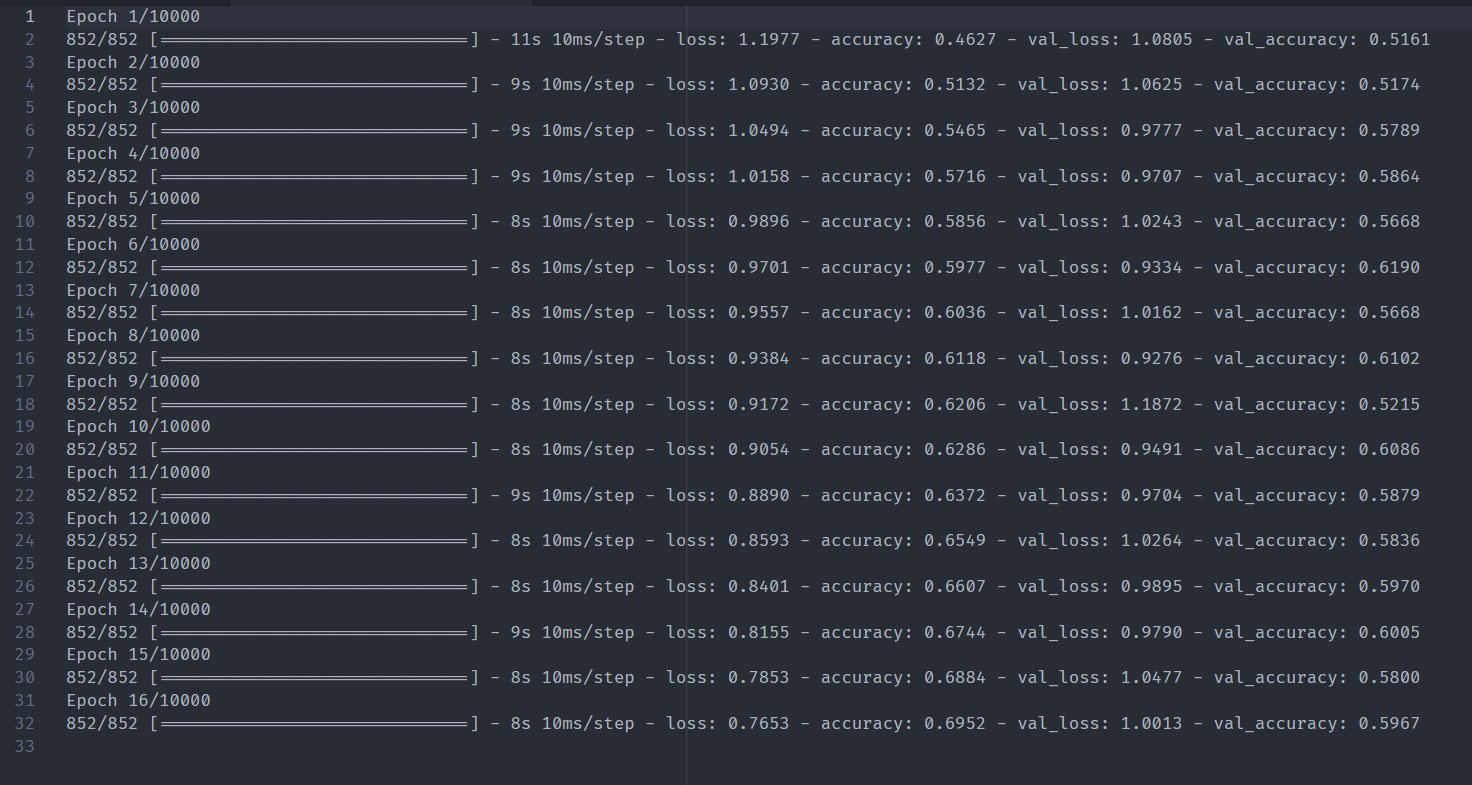
\includegraphics[width=\linewidth]{Pictures/CNN_Model/5_class_training_log.jpg}
    \caption{Training Log for the 5-class Classification Model}\label{fig3:5_class_log}
\end{figure}

Here we can see that as Training Stopped at epoch 16, our best model was in epoch 6 which had a validation accuracy of 61.90\%

\newpage

After some trial and error, we found that the best model 
we could make by altering the network size, had 2.7 million 
parameters for the five-class classification and 20.4 million 
parameters for the four-class model

\begin{figure}[h!]
    \centering
    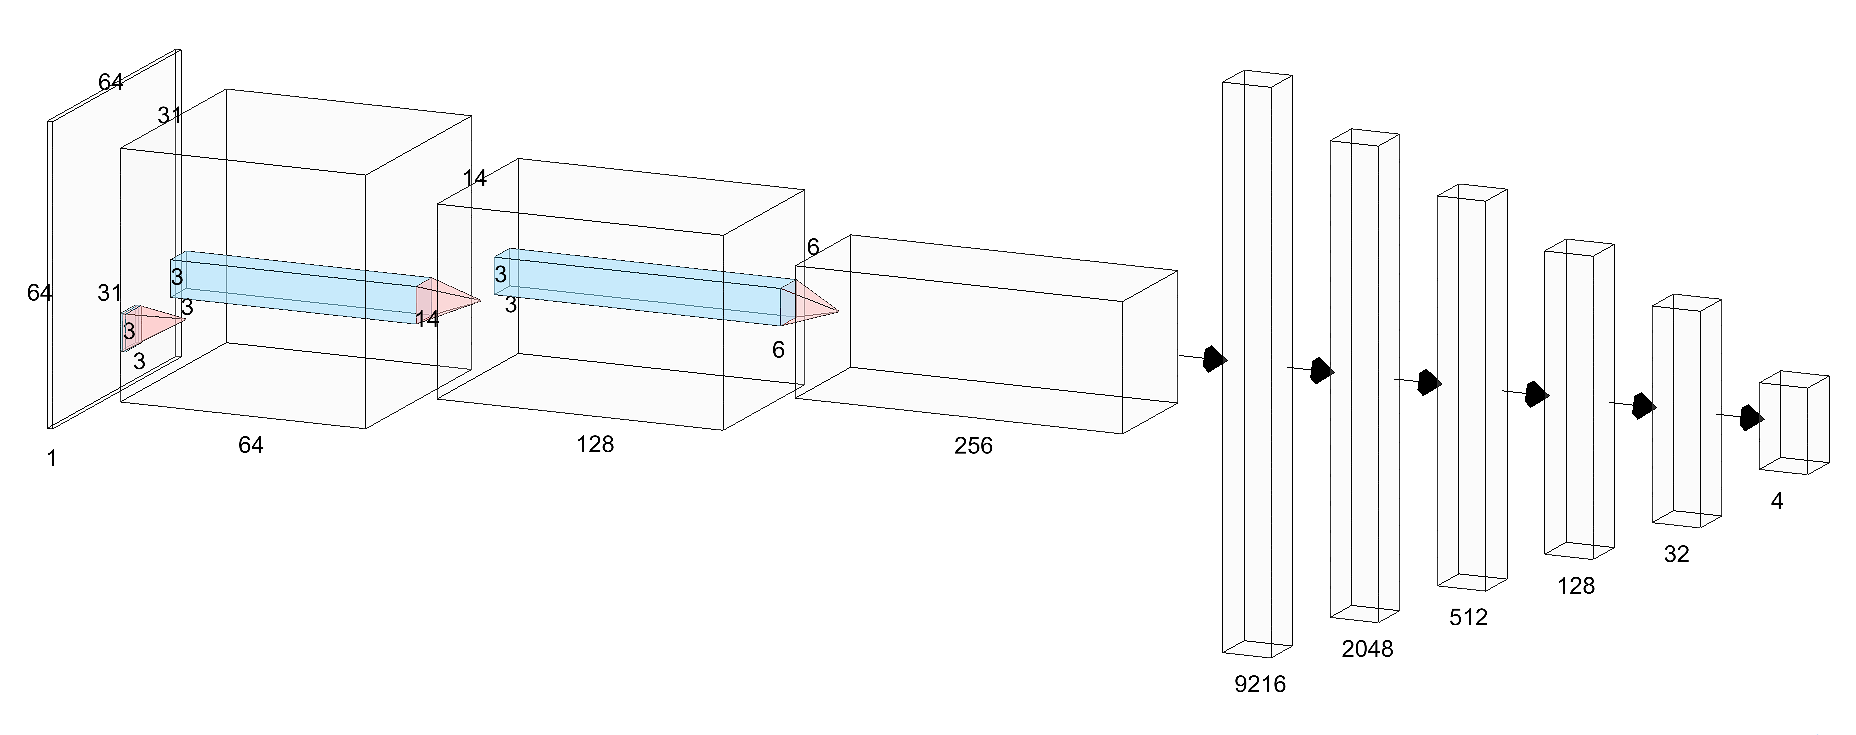
\includegraphics[width=\linewidth]{Pictures/CNN_Model/4_class_net_diagram.png}
    \caption{Model Diagram for 4 Class Classifier}\label{fig4:4_class_net}
\end{figure}

\begin{figure}[h!]
    \centering
    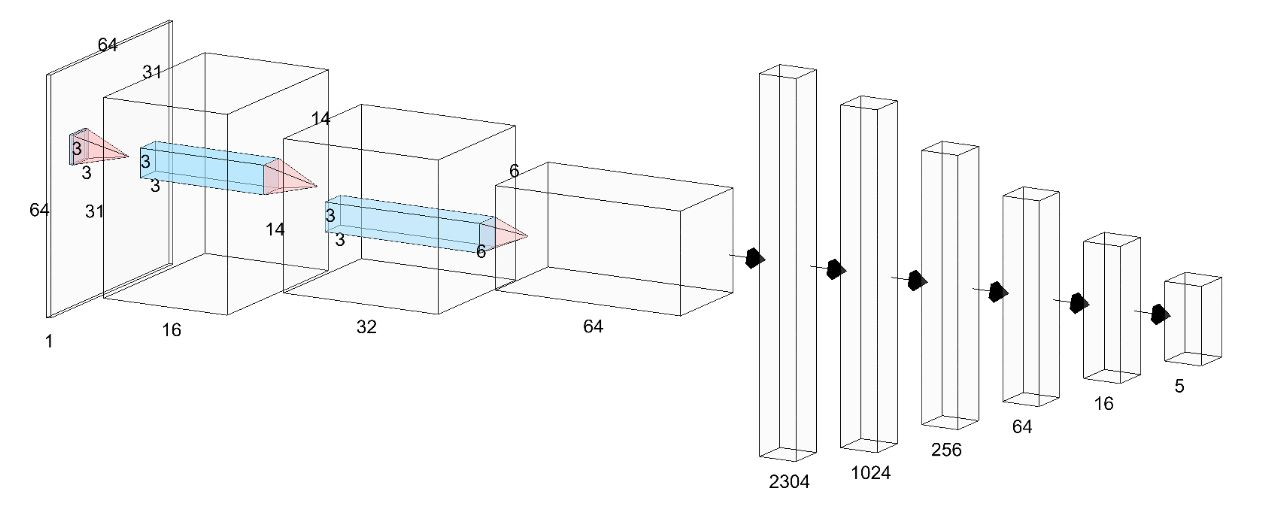
\includegraphics[width=\linewidth]{Pictures/CNN_Model/5_class_net_diagram.jpg}
    \caption{Model Diagram for 5 Class Classifier}\label{fig5:5_class_net}
\end{figure}

We were getting the test accuracy \textbf{60.71\% for four class classifier 
and 60.24\% for the five-class classifier}

\subsection{Model using Transformer}

Here we used GPT-neo with 125 million parameters and fine-tuned 
it with our generated dataset.

Our dataset consisted of 34075 rows that were split for training, 
testing, and validating in the ratio 80:10:10. The following 
are the sizes for each split:
\begin{itemize}
    \item Train dataset: 27260 rows
    \item Validation dataset: 3408 rows
    \item Test dataset: 3407 rows
\end{itemize}

\newpage

In the beginning, each of our input prompts is converted into 
tokens using GPT2 tokenizer. 

\begin{figure}[h!]
    \centering
    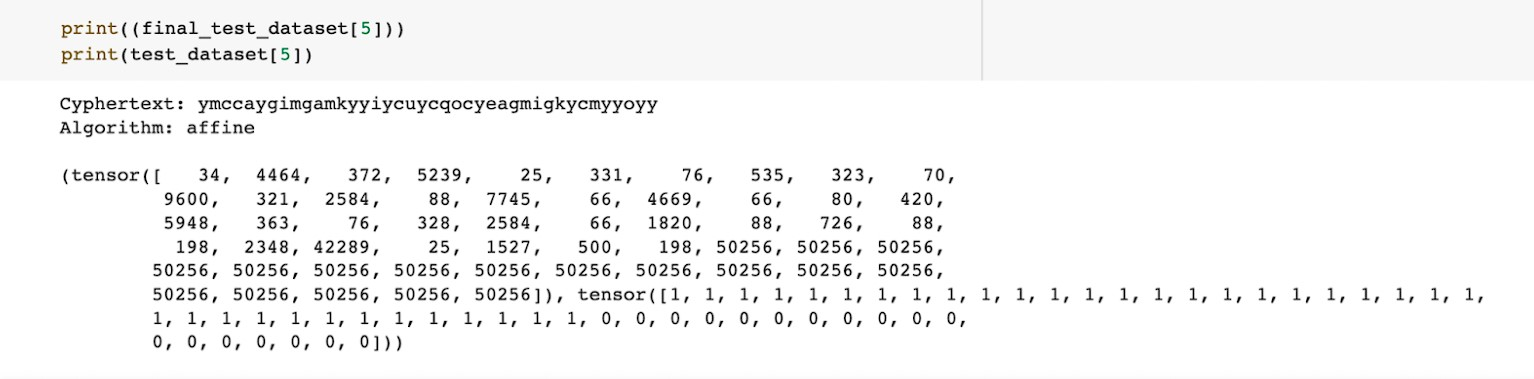
\includegraphics[width=\linewidth]{Pictures/Transformer_Model/text_tokenizer.jpg}
    \caption{GPT2 Tokenizer in action}\label{fig6:text_tokenizer}
\end{figure}

Here we see that the input prompt containing ciphertext and 
result has their corresponding tokens. Since we have used a 
tokenizer of fixed size, the unused indexes have higher integer 
values and have been masked by an attention mask containing 0 
at that index.

The training and validation data was fit into the model each 
having a batch size of 32 and was run for 5 epochs.
\begin{figure}[h!]
    \centering
    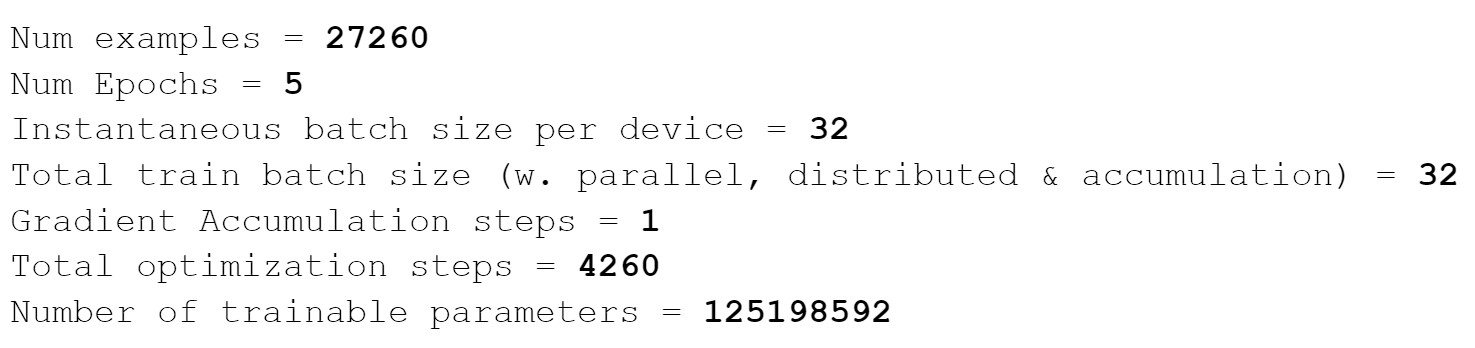
\includegraphics[width=0.8\linewidth]{Pictures/Transformer_Model/transformer_train_params.jpg}
    \caption{Training Parameters for the GPT-Neo Fine Tuning}\label{fig7:gpt-neo_params}
\end{figure}

\begin{figure}[h!]
    \centering
    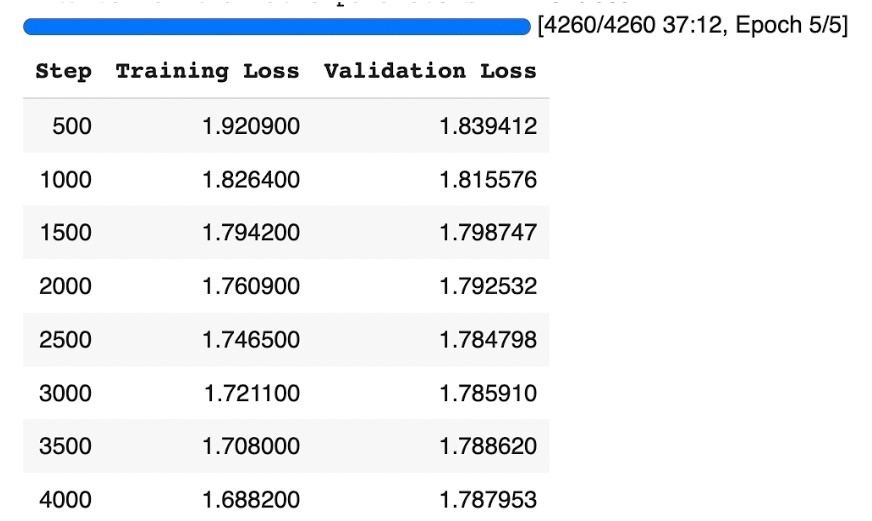
\includegraphics[width=0.5\linewidth]{Pictures/Transformer_Model/transformer_train_res.jpg}
    \caption{Training and Validation Loss obtained every 500 steps}\label{fig8:gpt-neo_train}
\end{figure}

After fine-tuning, we tested the model on our test dataset containing 
3407 rows. The model has shown an \textbf{overall accuracy of 85.236\%}.

\begin{figure}[h!]
    \centering
    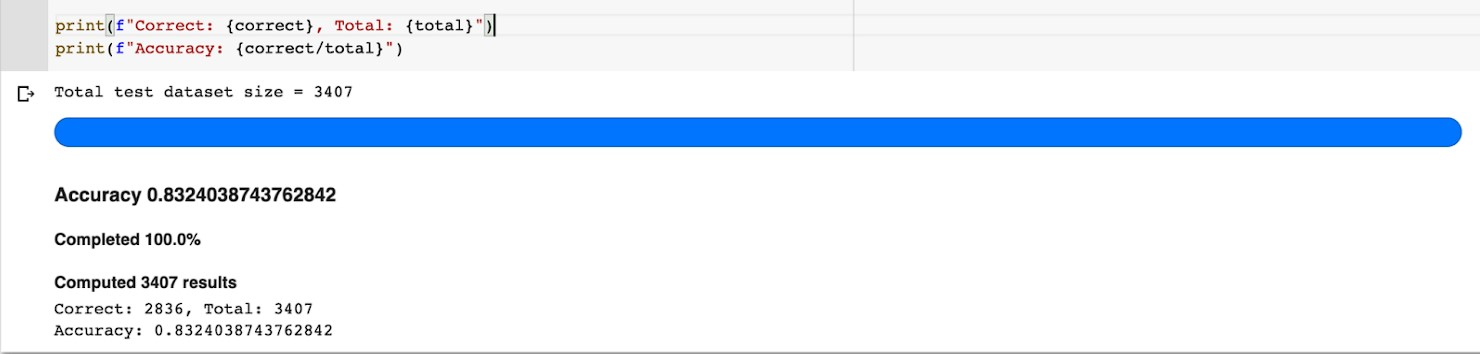
\includegraphics[width=\linewidth]{Pictures/Transformer_Model/transformer_test_res.jpg}
    \caption{Testing Accuracy for the Fine-Tuned GPT-Neo Model}\label{fig8:gpt-neo_test_res}
\end{figure}

\newpage

\section{FUTURE}

We would also like to alter the test to “image” conversion for 
the dataset to make CNN model perform better as it is not performing 
up to the standards that we want.

We would like to finetune our models to see if we can increase 
the accuracy. We are also curious to see if we can use an RNN 
instead of transformers and record the difference in accuracy 
of the two.

A similar analysis can be performed on other models such as:
\begin{itemize}
    \item OPT
    \item BERT
    \item GPTJ
    \item Bloom
\end{itemize}

Apart from this, we would like to explore feature detection 
to create a model and compare this approach with the transformer-based 
model.

Once we are satisfied with the model accuracy on 5 classes of 
ciphers, we would like to extend the model to detect more classes 
such as AES, DES, RSA, etc.

\section{\textcolor{red}{CONCLUSION}}

This report shows the current progress of our work in the detection of ciphertext using Artificial Neural Networks. Here we used two types of Neural Networks to achieve our objective, namely: Convolution Neural Networks and Transformer approach. 
\\

With the CNN approach, our model was able to achieve an accuracy of 61.90\% for 5 class classifications. We saw a significant improvement with the transformers approach on the same dataset and classes giving an accuracy of 83.24\%. This was primarily due to the higher number of parameters of Gpt-neo and the ability to memorize the local importance of tokens due to the self-attention feature. 
\\

In future work, we would like to extend the number of classes of ciphertext and also increase our dataset to find how our models perform in the new environment. We would like to try a feature-learning approach and also use more transformer models.  We would also like to solve the Cipher ID challenge from Mystery Twister C3  consisting of 500 ciphertexts. Based on our results and improvements, we would like to publish our work in a journal to see how our results stand in global competition. 


\newpage
\renewcommand{\refname}{REFERENCES}
\bibliographystyle{ieeetr}
\bibliography{mp}

\end{document}